\documentclass[11pt]{article}
% Default margins are too wide all the way around. I reset them here
\setlength{\topmargin}{-.5in}
\setlength{\textheight}{9in}
\setlength{\oddsidemargin}{.125in}
\setlength{\textwidth}{6in}

\usepackage{url}
\usepackage{amsmath}
\usepackage{color}

\newcommand{\textred}[1]{\textcolor{red}{#1}}
\ifx\noeditingmarks\undefined
  \newcommand{\pgwrapper}[2]{\textbf{#1: }\textred{#2}}
\else
  \newcommand{\pgwrapper}[2]{}
\fi
\newcommand\todo[1]{\textcolor{red}{#1}}
\newcommand\RED[1]{\textcolor{red}{#1}}
\newcommand\BLUE[1]{\textcolor{blue}{#1}}
\newcommand\GREEN[1]{\textcolor{brown}{#1}}
\newcommand{\para}[1]{\smallskip\noindent {\bf #1}}

\begin{document}
\title{Agent: Find Your Expert}
\author{
  Brandon Li\\
  Chris Zheng \\
  Daniel Tahara\\ \\
  {\it Yale University}\\
  \{brandon.li, chris.zheng, daniel.tahara\}@yale.edu
}
\renewcommand{\today}{}
\maketitle

\section{Introduction}
\label{sec:intro}
As people increasingly eschew traditional, physical information sources such as
books and television, they turn to internet for information of all forms,
whether they be tutorials, videos, or encyclopedia entries. Yet as they turn to
the internet for its ease of use, they increasingly expect curated or summarized
content instead of the original source material. This has manifested itself in a
number of ways. One trend we have seen is the proliferation of free,
question-and-answer sites (let alone message boards and other sites).  Yahoo
Answers~\cite{yahoo} is among the most well of these sites, allowing users to
post arbitrary (not necessarily fact-based) questions to which anyone can
respond. Of course, in exchange for ease of use and a broad audience comes a
large amount of noise and spam, so other companies have a) created
domain-specific, micro-sites sites like those in the StackExchange\cite{stackx}
network, and/or b) augmented the question-and-answer model with an extensive
reputation system, so that only reputable and qualified users can respond to
questions (examples include StackExchange sites as well as Quora~\cite{quora}).

However, just as these sites because of their abilities to reach large
audiences, so too do they fall short because of the inability to communicate
synchronously (e.g.\ to clarify an explanation) and the lack of any real
incentive for individuals to provide content. Thus, we have also seen the
development of paid information retrieval services such as
Cha-Cha~\cite{chacha}, kgb~\cite{kgb}, and even the commodotization of those
services through sites such as Amazon's Mechanical Turk~\cite{turk}.

A fundamental limitations of question-and-answer sites (and even the internet as
a whole) is that while it is a nearly infinite repository of information, it
does not, and perhaps cannot, capture the full extent of knowledge---the
understanding of information and associations between things---of the
contributing users. Projects such as IBM Watson~\cite{watson} and Google
Knowledge Graph~\cite{knowledge}, as well as the development of the Resource
Description Framework~\cite{rdf} are a step toward a knowledge-based, semantic,
web, but their usefulness is limited to certain, well-defined tasks.

Enter Agent. Rather than automating the process of knowledge gathering, Agent
identifies the individuals within your social networks who are most likely to be
able to provide knowledge about a particular topic. By recommending experts
from people you actually know, Agent improves your ability to get a timely,
personal response, and allows you to establish a more meaningful dialogue about
a topic than allowed by one-off, question-and-answer formats or pre-written
articles. Agent brings you knowledge through the web.

\section{Features}
\label{sec:features}
The core functionality of Agent is quite simple. Given a question or search
string, it identifies people in your social networks who might best be able to
provide you knowledge on that topic. A typical usage pattern might be the
following:
\begin{enumerate}
\item Log in or create an account
\item Link account to data sources (Facebook, LinkedIn, Twitter, etc.)
\item Ask about a topic by filling in one of the template questions (e.g.\ ``I
want to learn about XXX'' or ``I want to travel to XXX'')
\item View sorted list of connections who are likely to be able to answer your
question.
\end{enumerate}

Possible extensions could include integrating with messaging platforms on the
various linked accounts, so that you can ask your question immediately and track
responses to those questions. Additionally, we can generalize the set of
questions that a user can ask. This would involve doing semantic analysis of the
question in order to identify the information the user is looking for.

\section{System Architecture and Implementation}
\label{sec:architecture}

\begin{figure}[!h]
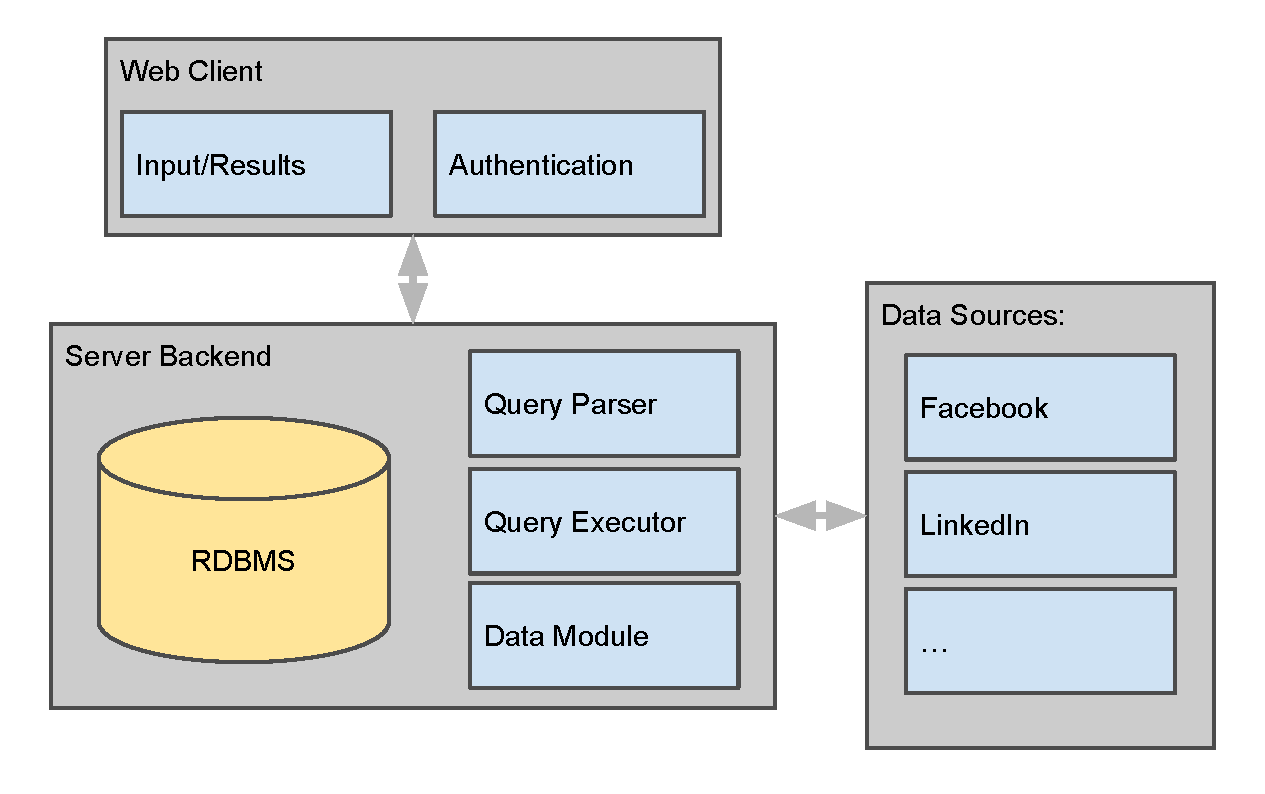
\includegraphics[width=\linewidth]{figs/sysarch.pdf}
\caption{Agent System Architecture}
\label{fig:sysarch}
\end{figure}

Our system architecture is shown in Figure~\ref{fig:sysarch}. At the highest
level, Agent comprises three components, a web client, a server backend, and set
of data sources. We discuss each in turn, with an eye toward demonstrating how
data flows through the system.

\subsection{Web Client}
The web client, as the user-facing component of the application, is responsible
for capturing user input to pass to the server backend  It is implemented as a
series of models and views using the Python Django framework.

\subsubsection{Input/Results}
\todo{Chris of BLi, please fill in once this is done}

\subsubsection{Authentication}
The web client authenticates users by using the Facebook OAuth API. Although the
current implementation of Agent does not persist user information across
sessions and therefore does not have `accounts,' an account would be implemented
by associating a unique user id with a given facebook OAuth token. A user would
then `link' to other data sources (described below) using their corresponding
APIs. These references would be stored in a table that associates each of these
data sources (Facebook included) with the unique user id for the given account.

\subsection{Server Backend}
The server, like the client, is built as part of a Django application. It is
composed of a number of modules, most of which are built into the application
models and others of which are implemented as standalone utilities.

\subsubsection{Query Parser}
The query parser receives text queries from the web client and resolves them
into sets of entities through a term extraction process. At a high level, it
identifies tags by measuring the likelihood that the words in the query co-occur
and whether their co-occurence in the input is `important' (one measure for
determining this is pointwise-mutual information\footnote{See:
http://www.eecis.udel.edu/~trnka/CISC889-11S/lectures/philip-pmi.pdf} Currently,
we rely on the Yahoo Content Analysis API to tag entities~\cite{yahoo_ca}, but
we could use any reasonable term extraction module in order to determine our
final query form. A more complex, customized term extraction algorithm might
improve our results, but this diverges into linguistics and formal semantics, so
we do not pursue this option in our current implementation.  Furthermore, if we
extended Agent's functionality to accept arbitrary questions (rather than
templated questions), a layer of semantic analysis would be necessary. Again, we
see this as more of a linguistics problem, so we leave it as a potential
extension of the current system.

\subsubsection{Query Executor}
The query executer receives a set of entities from the Query Parser and then
generates the database queries necessary to `score' each connection in the
user's social network.  It then returns the $N$ (a user-configurable parameter)
connections with the highest score.  The score corresponds to the likelihood
that the connection might be able to answer the inputed query. Agent's scoring
algorithm and the corresponding SQL are presented in Section~\ref{sec:scoring}.

In our implementation, the SQL is actually generated on-the-fly by the Django
framework. Our interface to the data is therefore through the models API rather
than through the underlying RDBMS.

\subsubsection{Data Module}
The data module is responsible for retrieving data from each of the user's
linked data sources and transforming that data into the end format utilized by
our RDBMS (we call these data {\it interactions}). Agent's data model and ETL
process are detailed in Section~\ref{sec:data}. The module is implemented as a
collection of Python utilities.

\subsubsection{RDBMS}
The RDBMS is responsible for persisting account information (the set of linked
accounts associated with a given user id) as well as the set of interactions for
each connection. These interactions are the target of Agent queries. The RDBMS
therefore interacts with both the Query Executor and Data Module. Agent uses
Postgres as its RDBMS.

\subsection{Data Sources}
The data sources are any social networking sites that define users and
connections among users, along with a profile or set of actions that a user can
perform. In the current implementation, we support Facebook as a data source,
but this is easily extensible to sites such as LinkedIn and Tumblr. Agent
accesses the data sources using the credentials provided during authentication
through the REST APIs offered by each source. For each site, we implement a new
ETL module to transform the data to our target format (described in
Section~\ref{sec:data}).

\section{Data Model and ETL}
\label{sec:data}
Given the disparate object models of the data sources that Agent utilizes, it is
necessary to transform data from the original format to a single, source
independent format over which the query executor can operate. This section
defines this target data model and details the ETL process.

\begin{figure}[!h]
\begin{center}
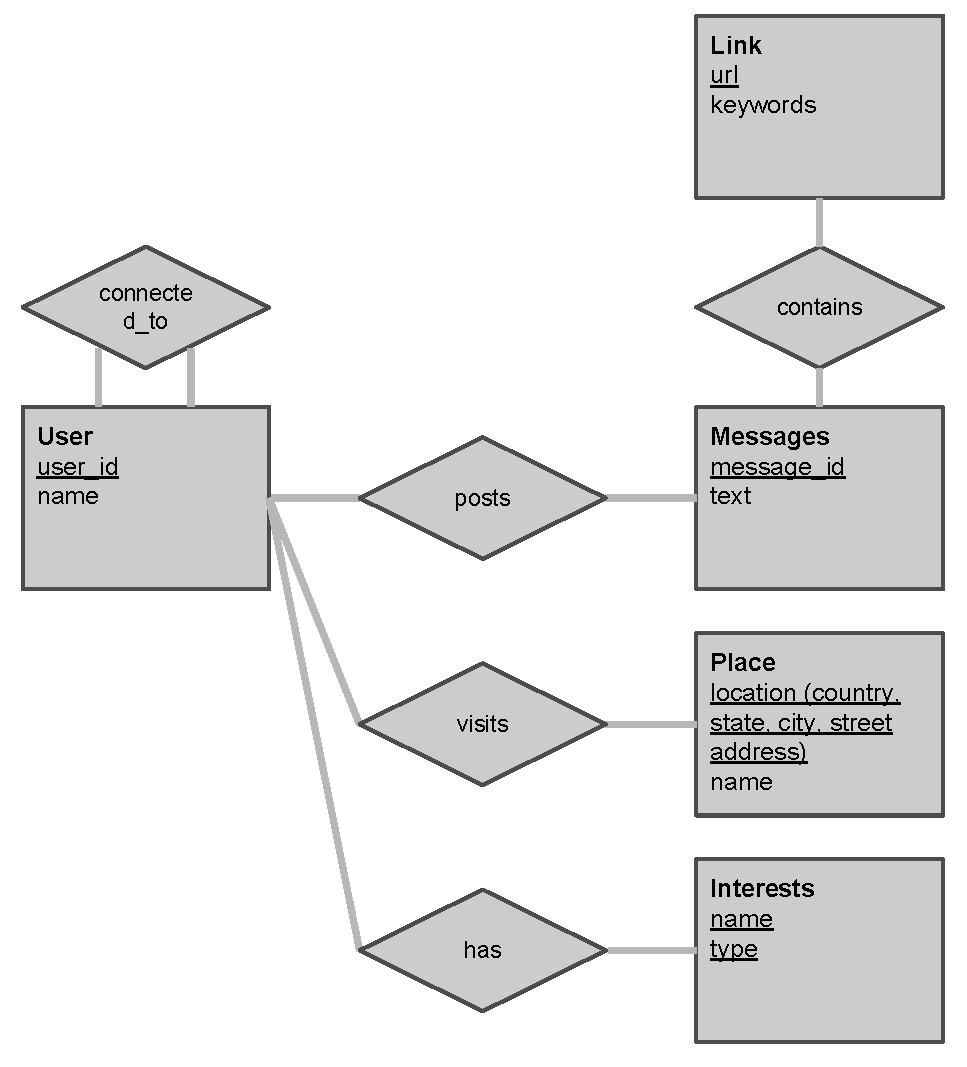
\includegraphics[width=0.5\linewidth]{figs/er-datasource.pdf}
\caption{Entity-Relationship Diagram for Data Sources}
\label{fig:er-datasource}
\end{center}
\end{figure}

We represent social networking data using the Entity Relationship (ER) diagram
shown in Figure~\ref{fig:er-datasource}. Conceptually, we characterize this data
as a set of users and set interactions. Users can be connected among themselves,
and Agent uses those connections to identify candidates for answering a given
query. Interactions are more variable across sites, but on a high level, we
classify them as either posts, profile elements (supplied, structured
information), or locations. The exact mapping of API response objects to these
interaction types varies by site, and furthermore, a single response object
(e.g.\ a Facebook post) might map to multiple interactions (both a post and
location). Agent's backend has a module per data source and performs the mapping
accordingly.

\begin{figure}[!h]
\begin{center}
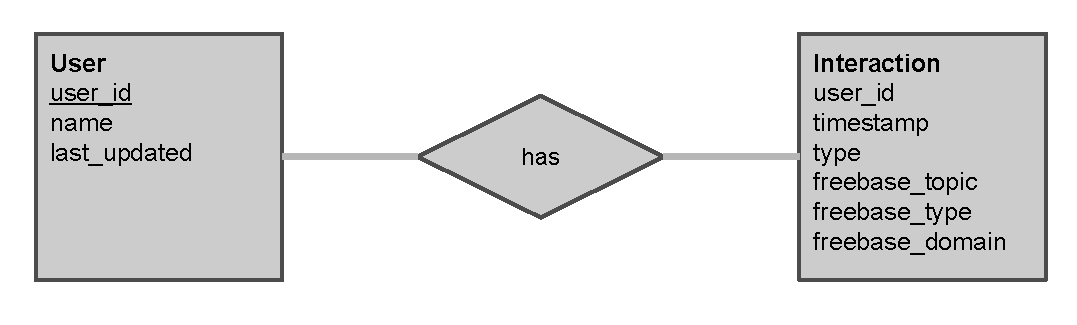
\includegraphics[width=0.5\linewidth]{figs/er-agent.pdf}
\caption{Simplified Entity-Relationship Diagram for Agent Backend}
\label{fig:er-agent}
\end{center}
\end{figure}

Our target data model is shown in Figure~\ref{fig:er-agent}. Note that we have
simplified it for the sake of discussion, representing each of posts, profile
elements, and locations by their superclass, interaction. In practice, we
maintain separate tables for each interaction type, which enables us to more
easily change the information that we store per interaction type as well as to
modify the scoring algorithm.

As shown in the Figure, Agent represents each interaction by the associated
user, a timestamp, and then a collection of Freebase identifiers. Freebase is
``a community-curated database of well-known people, places, and things'' that
represents its entities as nodes in a graph connected to each other by various
properties \cite{freebase, freebase-api}. Most importantly, Freebase taxonomizes
each entity by a domain and a type (actually a set of them), which allows users
to classify topics by knowledge area, a perfect fit for our application.

Although our current implementation of Agent uses Freebase identifiers, Agent is
not dependent on Freebase. Agent could very easily use Wikipedia or
other identifiers or even a custom knowledge representation format. However,
Freebase is particularly convenient and well-supported and therefore a good
choice for use in our application.

Given the data models described above, the ETL process is straightforward. Given
an API response, the data module generates a set of {\it user\_id, timestamp,
interaction\_type, entity} tuples. The entities are extracted from the original
response object based on the objects format. For example, profile elements are
usually limited to entities recognized by the social networking site, so the
entity mapping is simply the API response. On the other hand, a post generally
contains a string of text, so the data module performs term extraction
similarly to the query parser (see Section~\ref{sec:query-parser}).

After generating the intermediate tuples, the data module takes those tuples and
generates a final set of tuples with the attributes shown in
Figure~\ref{fig:er-agent}. Specifically, given an entity, the data module uses
the Freebase search API to generate a candidate list of Freebase topics, and
then selects the most likely topic. It then retrieves that topic's type (or in
the event that the topic falls under multiple types, the most notable one) and
similarly its domain. This data is then combined with the other input and stored
as a tuple in the appropriate table in the database, based on the interaction
type.




\section{Scoring Algorithm}
\label{sec:scoring}

Many recommendation systems today can be classified as either content-based
systems or collaborative filtering systems
\cite{recsys}. Content-based systems seek
to offer you suggestions based on items a user has already given some form of
feedback on, while collaborative filtering systems search social graphs to find
people who would have similar ``taste'' to a given user and make recommendations
based on these similar users. Usually, these types of recommendations present
themselves as ``items like X'' or ``similar users also purchased/likes X,''
respectively. Since Agent is responding to specific queries rather than drawing
similarities between users, we decided that a content-based approach was more
appropriate.

In using a content-based system, we had to design a scoring algorithm in order
to rank different candidates in response to the query. At a high level, we
identified the identified the scoring criteria as follows:
\begin{enumerate}
\item Frequency of search keys in friend's activity
\item Frequency of related terms in friend's activity
\item Priority to ``specialized'' terms
\item Priority for more search keys matched
\end{enumerate}
where friend's activity includes a user's profile information, statuses, and likes
and ``related terms'' are defined as the topic and domain of a term as given by the Freebase API.


\begin{algorithm}
\caption{Score Friend}
\begin{algorithmic}
\STATE Assume we have $friendId$ and $\alpha > \beta > \gamma$
\STATE $score \gets 0$
\FORALL{$key \in search-keys$}
  \FORALL{$entity \in entities_{userId=friendId}$}
    \IF{$entity[``mid''] = key[``mid'']$}
      \STATE $score \gets score + (\alpha \times tfscale_{entity})$
      \STATE continue
    \ENDIF
    \IF{$entity[``typeMid'']  = key[``typeMid'']$}
      \STATE $score \gets score + (\beta \times tfscale_{entity})$
      \STATE  continue
    \ENDIF
        \IF{$entity[``domainMid'']  = key[``domainMid'']$}
      \STATE $score \gets score + (\gamma \times tfscale_{entity})$
      \STATE  continue
    \ENDIF
\ENDFOR
\ENDFOR
\STATE Scale score by number of keys matched
\end{algorithmic}
\end{algorithm}

Term Frequency Inverse-Document Frequency (TF-IDF) \cite{tfidf} is a
well-established metric for determining how relevant a given term is to a
document. It is based off of a ``relative frequency'' count of the search key
and is scaled by how common the word is in general. However, based on this
measure, a document can only be highly relevant for a few topics, whereas we
believe some people are simply more equipped to answer more questions than
others, based on the size of their knowledge set. Therefore, for criteria 1 and
2, we opted for an absolute frequency instead of a relative frequency.
Specifically, we looked at the number of times that the search keys (or related
terms) appear in the person's Facebook activity.

A concept that we did adopt from TF-IDF is the idea of prioritizing
``specialized'' terms. The motivation behind this is two-fold: \begin{enumerate}
\item Words that are used more commonly will otherwise dominate the score, and
thus the counts of these words should be offset
\item We suspect that the more ``specialized'' search keys are more definitive
of the user's query.
\end{enumerate}

We calculate ``specialized'' words by how frequently they have appeared in past
searches or in the activity of any user in our database.

As for the fourth criteria, we seek to recommend ``experts'' based on how well
they match a query, so if only part of a query is matched, we consider that to
be less good of a match than a user who matches all parts of a query. If the
user was only interested in a subset of their query, they simply could have
searched for that subset.

Given that our service is in essence a ``friend filter,'' these criteria were
selected based on what a user might expect this service to be doing. There is very
little emphasis on ``discoverability.'' We are simply helping the user parse
through a lot of data and quickly find the friends that match a search query
in a way that is transparent and intuitive to them.

In terms of choosing the scaling factors, we had the option to use a
machine-learning approach to optimize over a certain condition, but there is no
really sensible condition for which we can rank to relative importance of these
various criteria, especially because we are not collecting any ratings values
from the users. It is also generally difficult to claim the effectiveness of a
recommendation system strictly using a quantitative measure. Thus, we selected
our parameters through testing runs using different parameter values for our
algorithm and choosing the set of parameters for which the users had the most
positive response. Although, in the future, it might be interesting to adjust
the parameters.


\section{Implementation}
\label{sec:implementation}

We implemented our system using the Python Django framework

- Tagging and entity extraction - Yahoo...
- End format - freebase topics
- separated into tables means we can store different information/adapt our
scoring
- Postgresql


Basic user flow

\section{Conclusion}
\label{sec:conclusion}

\bibliographystyle{plain}
\bibliography{ref}
% That's all folks!
\end{document}

